\chapter{提案手法}
\label{proposed}



\begin{figure}[hbtp]
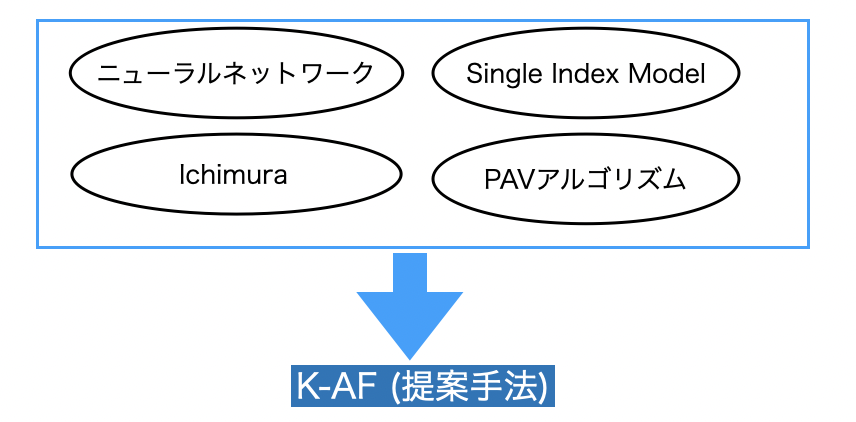
\includegraphics[width=15cm]{asset/proposed_method.png}
	\caption{提案手法}
	\label{proposed_method}
\end{figure}


本章では背景で述べた課題を整理しつつ、それらを解決する提案手法の位置付けについて述べる。
\ref{history_activation}では既存の活性化関数の動向を踏まえながら本提案手法へとつながる過程を述べる。
次の章で私が提案する活性化関数の数式について解説する。
次の章でそのアルゴリズムについて解説する。



\section{活性化関数と背景}
\label {history_activation}


\begin{figure}[hbtp]
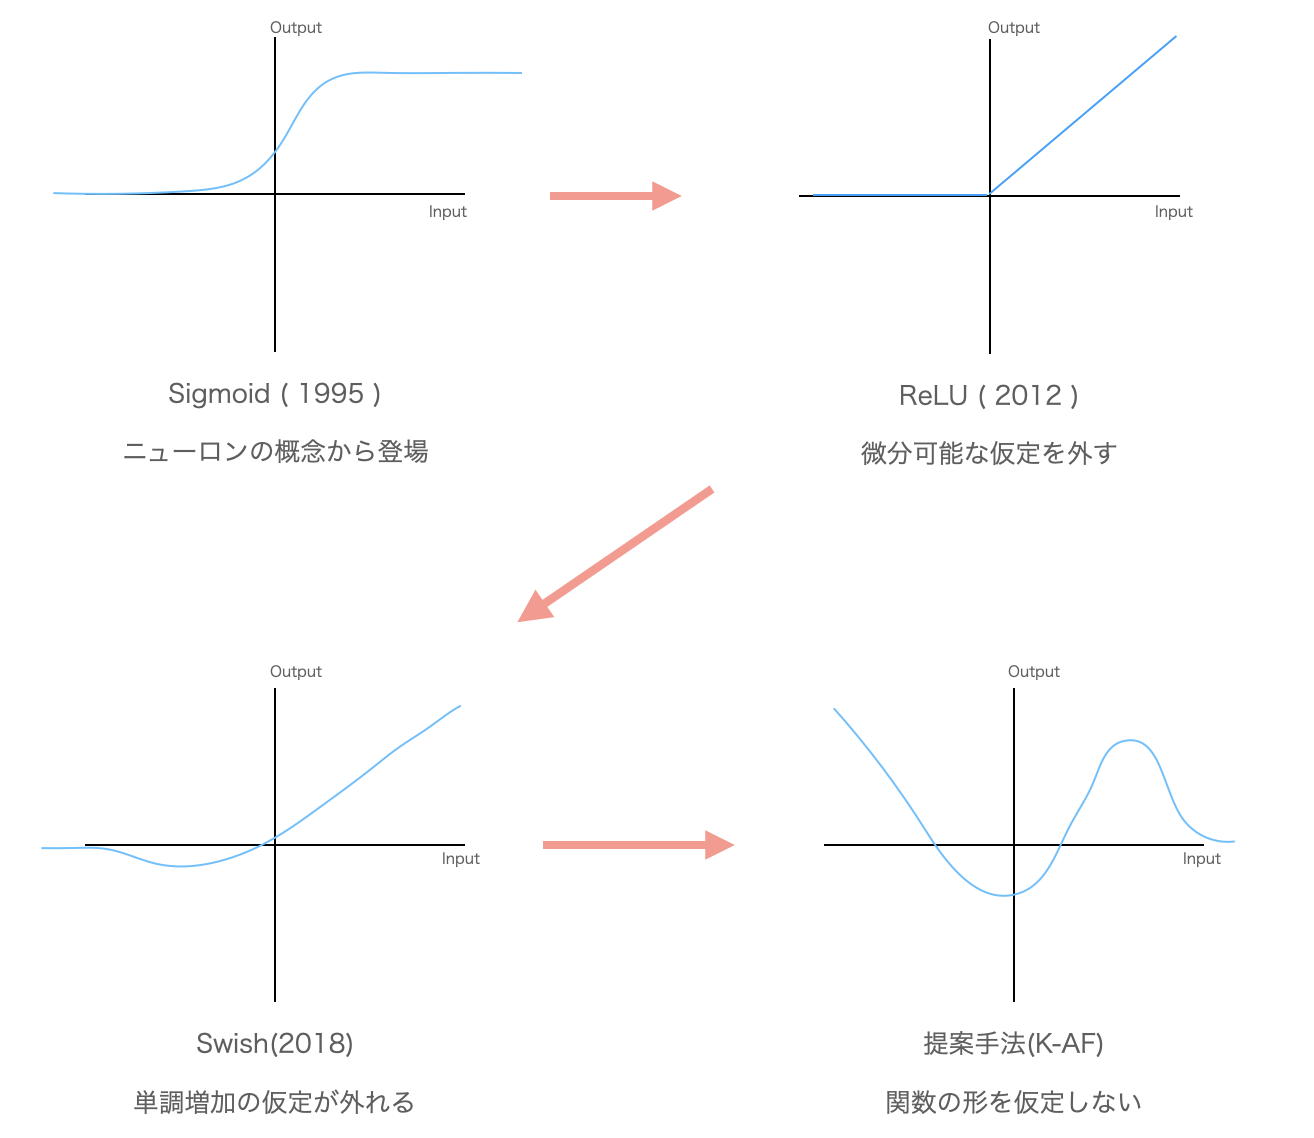
\includegraphics[width=15cm]{asset/history_af.png}
	\caption{活性化関数の歴史}
	\label{history_af}
\end{figure}

現在、深層学習に利用できる活性化関数が研究されている。特に近年では、中間層にReLUを用い出力層にSigmoid関数を用いた組み合わせがよく用いられている。
しかし、これらの組み合わせは経験的なものだけでなく、データに対する人間の知識が事前に必要とされる。

また、本研究で提案する活性化関数はSwishやMishなどからの単調増加性の仮定を外した点に着目した。
Sigmoidはロジスティック回帰から生まれたものであり、ReLU自体も実験的に精度がいいと導出されただけのものであった。
それらの単調増加性という性質は機械学習の観点では本来必要ではないと考えることもできる。
図\ref{history_af}のように、活性化関数はSwishやMishなどといった形へと進化する中で、単調増加性を仮定する必要がなくなった。
isotonic regression同様に単調増加性について仮定しているようであるが、本研究からはその仮定を外す。
そうすることで、より精度の高い結果を導き出すことができると予想される。
関数の推定はカーネル密度推定で行う。
これにより活性化関数を既存の関数から選択するのではなく、関数空間全体から活性化関数を推定することができる。
これにより、これまでディープラーニングで課題とされてきた活性化関数の選択の問題を解決することが可能となり、新たなアプローチが可能になることが予想される。
また、これまで選択してきた活性化関数が実験的に正しいかどうか判定することも可能であると考えられる。


\section{提案手法の位置付け}

本研究の提案手法の位置付けをまとめた図を\ref{proposed_method}に示した。
統計学の世界でSingleIndexModelにおけるIchimuraの手法を多次元化し、学習アルゴリズムにPAVアルゴリズムを組み合わせた手法をニューラルネットワークの活性化関数に応用する。



\section{K-AF}
本論文で私が提案する活性化関数を以下の数式で表現する。


\begin{eqnarray}
G(X_iw)=\frac{\sum_{i\neq j} K\left(\frac{X^{calc}_j w - X_i w}{h_{calc}}\right)Y^{calc}_j}{\sum_{i\neq j} K\left(\frac{X^{calc}_j w - X_i w}{h_{calc}}\right)}
\label{eq:k-af}
\end{eqnarray}

~\cite{ichimura}ではデータセットの数だけで表現していたが、一部を省略することにより少ない変数で表現することに成功した。詳細な数式の導出はappendix\ref{appendix:calc}で述べた。
$ i \neq j $ にっている理由は過剰適合を抑えるためにleave one out 


\subsection{バンド幅推定}


\begin{figure}[hbtp]
    \begin{center}
            \begin{minipage}{0.40\hsize}
                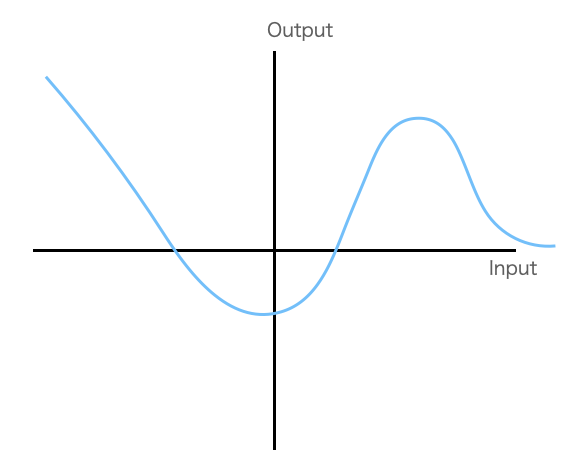
\includegraphics[width=5cm]{asset/k_af_band_big.png}
                    \caption{バンド幅が大きいと、K-AFで表現できる活性化関数の数は減る。}
                    \label{k_af_band_big}
            \end{minipage}
            \begin{minipage}{0.40\hsize}
            \hspace{10pt}
                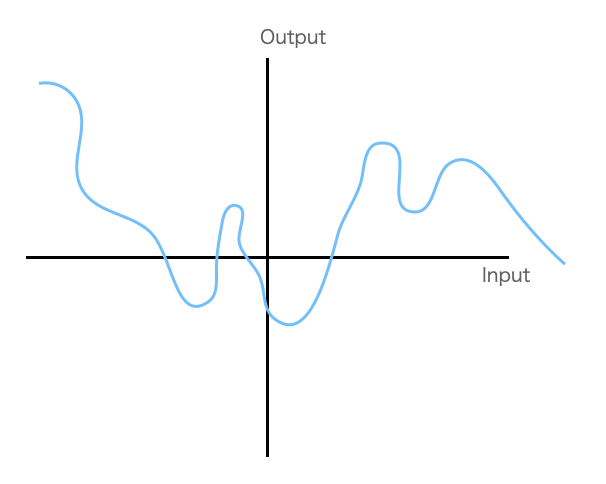
\includegraphics[width=5cm]{asset/k_af_band_small.png}
                    \caption{バンド幅が小さいと、K-AFで表現できる活性化関数の形は大きくなる。}
                    \label{k_af_band_small}
            \end{minipage}
    \end{center}
\end{figure}


カーネル密度推定は関数の形状を推定するにあたってバンド幅の大きさが非常に重要になる。
バンド幅は大きいほど関数の自由度が減り、小さいほど自由度が大きくなることが容易に推定できる。

\ref{k_af_band_small}の方が表現の幅が広いが、勾配消失の問題や過学習の問題が考えらる。
本実験ではこのバンド幅も学習のパラメータに含めることで最適なバンド幅を推定できるようにした。

\section{アルゴリズム}

入力の次元をd


\begin{algorithm}[]
	\caption{\KAF}
	\label{alg:fixed-u-alg}
\begin{algorithmic}
	\STATE {\bfseries Input:} data $\langle (x_i, y_i) \rangle_{i=1}^m \in
	\reals^d \times [0, 1]$, $u: \reals \rightarrow [0, 1]$.
	\STATE $w^1 := 0$;
	\FOR {$t = 1, 2, \ldots$}
	\STATE $h^t(x) := u(w^t \cdot x)$;
	\STATE $w^{t+1} := w^t + \displaystyle\fraconem \sumionetom (y_i - u(w^t
	\cdot x_i)) x_i$;
	\ENDFOR
\end{algorithmic}
\end{algorithm}

これが実装のアルゴリズムである。pythonでの実装についてはappendix\ref{appendix:algorithm}に記述した。
いかにアルゴリズムの手順を記す

\begin{itemize}
  \item 出力層に使う活性化関数を状況に応じた適切な形に変わる汎用的な関数を導き、高い精度を出せるようにした。
  \item そのような関数を使うことで、データセットの形等の専門的な知識を理解しなくて済むようになり、ニューラルネットの構築を容易にした。
\end{itemize}



%%% Local Variables:
%%% mode: japanese-latex
%%% TeX-master: "../bthesis"
%%% End:
